%
\documentclass[a4paper]{scrartcl}

\usepackage{amsmath, amssymb}
\usepackage{graphicx}
\usepackage{natbib}
\usepackage{hyperref}
\hypersetup{pdfpagemode = {UseNone},
            pdftitle = {On the integrals of ellipses in the r-phi plane},
            pdfauthor = {Thomas Rometsch},
            pdfsubject = {},
            pdfview = {FitH},
            pdfstartview = {FitH},
            colorlinks = {true},
            linkcolor = [rgb]{0,0.35,0.7},
            citecolor = [rgb]{0,0.35,0.7},
            filecolor = [rgb]{0.61,0,0},
            urlcolor = [rgb]{0.61,0,0},
           }
%%%%%%%%%%%%%%%%%%%%%%%%%%%%%%%%%%%%%%%%
\usepackage{txfonts}
%%%%%%%%%%%%%%%%%%%%%%%%%%%%%%%%%%%%%%%%
\usepackage{enumitem}
\usepackage{placeins}



% %%%%%%%%%%%%%%%%%%%%%%%%%
% %%% Commenting System %%%
% %%%%%%%%%%%%%%%%%%%%%%%%%

\usepackage{lineno}
\linenumbers


\usepackage[dvipsnames]{xcolor}



\begin{document}

\title{Integrals over ellipses defined in the $r-\phi$ plane}

\author{Thomas Rometsch}

\date{\today}

\maketitle
%
%________________________________________________________________



Vortices in protoplanetary disks appear as banana-shaped object in the disk.
However, in the $r-\phi$ plane, they have an elliptical shape.
The vortices can be identified by closed lines of constant vortensity, 
$\varpi = \frac{(\nabla \times \vec{v})_z}{\Sigma}$,
where $v$ is the velocity of the gas and $\Sigma$ the surface density.
To account for radial variation of $\Sigma$ and the Keplerian velocity profile of the disk,
it is advantageous to normalize the vortensity by the background vortensity, 
$\varpi_0 = \frac{(\nabla \times \vec{v}_\mathrm{Kepler}(r))_z}{\Sigma_0(r)}$
of the Keplerian flow divided by a background surface density profile.
Meaningful values of the resulting quantity $\frac{\varpi}{\varpi_0}$ can be expected to be in the range -1 to 1
for retrograde vortices.

Having identified a suitable ellipse in the $r-\phi$ plane, 
we can then define a vortex as the material enclosed by the ellipse.

These ellispes are described by their center coordinates, $r_0$, $\phi_0$, and their extents
$2h_r$ and $2h_\phi$.

Thus the ellipse equation takes the form

\begin{align}\label{eqn:ellipse_equation}
  \left( \frac{r - r_0}{h_r} \right)^2 + \left( \frac{\phi - \phi_0}{h_\phi} \right)^2 = 1
\end{align}

Without loss of generality, we can set $\phi_0 = 0$ by rotating the frame of reference.

Note, that the $\phi$ direction does not carry a unit of length.
The corresponding length is the distance on the arc at radius $r$.
This needs to be accounted for during integration of quantities over the ellipse.

The area of the ellipse in the $r-\phi$ plane does not carry physical meaning.
The physically relevant quantity is the area enclosed by the corresponding region in the disk.

In the $r$ - $s$ plane, where $s$ is the length on an arc along the azimuthal direction,
the ellipse in stretched for $r > r_0$ and pinched for $r < r_0$.
See the center panel of Fig.\,\ref{fig:geometries} for a sketch of this geometry.
The bounding lines indicated with $\phi=\pi$ and $\phi=-\pi$ identify the same line in the right panel
and represent a periodic boundary.

To calculate the area in the physically meaningful cartesian plane, 
we need to integrate in polar coordinates with the appropriate area measure,
where $r$ and $\phi$ must fulfill Eq. \eqref{eqn:ellipse_equation}.
The shape of the ellipse is not symmetric in cartesian coordinates, 
as can be seen in Fig.\,\ref{fig:geometries} in the center and right panels.
This is done by integrating from $r_0 - h_r$ to $r_0 + h_r$ in radial direction.
The azimuthal integration domain is $[-\alpha(r), \alpha(r)]$, where
$\alpha(r) = h_\phi \sqrt{1 - \left(\frac{r-r_0}{h_r}\right)^2}$ is defined by Eq. \eqref{eqn:ellipse_equation}.


\begin{align}
  A & = \int_{Ellipse} \mathrm{d}A
  = \int_{r_0 - h_r}^{r_0 + h_r} \int_{-\alpha(r)}^{\alpha(r)} r \mathrm{d}r \mathrm{d}\phi                \\
    & = 2 h_\phi \int_{r_0 - h_r}^{r_0 + h_r} \mathrm{d}r \, r \sqrt{1 - \left(\frac{r-r_0}{h_r}\right)^2} \\
    & = 2 h_r^2 h_\phi \int_{-1}^1 \mathrm{d}x \left(x + \frac{r_0}{h_r}\right) \sqrt{1-x^2}
  = 2 h_\phi h_r^2 \left( I_1 + \frac{r}{h_r} I_2 \right)
\end{align}

The substitution $r - r_0 = h_r x$ was and the integral was split in two parts.
The second integral disappears because the integrant is anti-symmetric, 
$  I_2 = \int_{-1}^{1} \mathrm{d} x\, x \sqrt{1 - x^2} = 0$.

The remaining integral can be identified as the area of a half-circle,
$I_1 = \int_{-1}^1 \mathrm{d} x \sqrt{1 - x^2} = \frac{\pi}{2}$.

Finally, the area in the cartesian plane appears to be equivalent to the usual formula with the extent $a_s = r_0 h_\phi$,
\begin{align}
  A = \pi h_r h_\phi r_0
\end{align}

A possible interpretation is that the stretching in the outer part is compensated by the pinching in the inner part.
See the center panel of Fig.\,\ref{fig:geometries} for how the shape is affected by the stretching and pinching.

\begin{figure}
  \begin{center}
    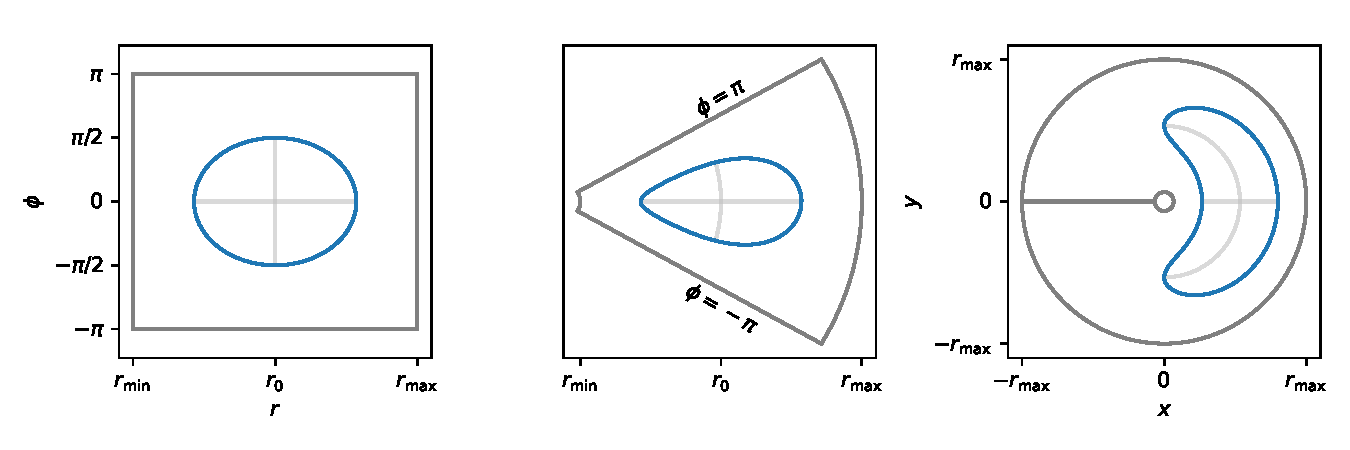
\includegraphics[width=\textwidth]{geometries.pdf}
    \caption{\label{fig:geometries}Illustration of the shape of a vortex which is defined in the $r-\phi$ plane.
    The panels show, from left to right, the shape of the vortex in the $r-\phi$ plane, 
    in a geometry where the disk is folded into a wedge shape, 
    and in cartesian coordinates, as it would be observed in a face-on disk.
    The light gray lines indicate constant $r$ and constant $\phi$ of the ellipse in the $r-\phi$ plane,
    and the darker gray lines indicated the boundaries of the disk.}
  \end{center}
\end{figure}

The definition for the vortex given above depends on the technicalities of how 
the lines of constant normalized vortensity are computed.
To give a precise definition for the vortex which , we fit bell curves to the surface density, $\Sigma$,
and the normalized vortensity, $\varpi/\varpi_0$.
The function is composed of two bell curves in radial and azimuthal direction as
\begin{align}
  f(r, \phi) = c + a \exp\left( - \frac{(r - r_0)^2}{\sigma_r^2} \right) \exp\left( - \frac{(\phi - \phi_0)^2}{\sigma_\phi^2} \right)\,.
\end{align}

Then the vortex can be defined as the region enclosed by an ellipse (in $r-\phi$)
with the extent is defined by the full-width-half-maximum of the bell curve, i.e. $h_r = \sqrt{2 \log(2)} \sigma_r$
and $h_\phi = \sqrt{2 \log(2)} \sigma_\phi$, or by some multiple of $\sigma_r$ and $\sigma_\phi$.
In general, any ratio $k = \frac{h}{\sigma}$ can be chosen.

Again, the physical relevant integrals need to be performed in the cartesian plane with limits defined by
the ellipse in the $r-\phi$ plane.
To evaluate the integral, we again rotate into a reference system such that $\phi_0 = 0$.
We will first split off the contribution from the constant part of $f$ by reusing the result for the area.

\begin{align}
  F & = \int_{Ellipse} f(r, \phi) \, \mathrm{d}A                                                
    = \int_{r_0 - h_r}^{r_0 + h_r} \int_{-\alpha(r)}^{\alpha(r)} r \,\mathrm{d}r \, \mathrm{d}\phi \,f(r, \phi)
    = A \,c + J \,,
\end{align}

\begin{align}
  J & = a \int_{r_0 - h_r}^{r_0 + h_r} r \,\mathrm{d}r \exp\left( - \frac{(r-r_0)^2}{2 \sigma_r^2} \right)
  2 \int_0^{\alpha(r)} \mathrm{d}\phi \exp\left( - \frac{\phi^2}{2\sigma_\phi^2} \right)   \,.
\end{align}

The $\phi$ integral can be evaluated using the error function, $\mathrm{erf}$, and the substitution
$y = \frac{\phi}{\sqrt{2} \sigma_\phi}$
\begin{align}
   & \int_0^{\alpha(r)} \mathrm{d} \phi \exp\left( - \frac{\phi^2}{2\sigma_\phi^2} \right)
  = \sqrt{2} \sigma_\phi \int_0^{\frac{\alpha(r)}{\sqrt{2} \sigma_\phi}} \mathrm{d}y \exp(-y^2)                                            \\
   & = \sqrt{\frac{\pi}{2}} \sigma_\phi \mathrm{erf} \left( \frac{h_\phi}{\sqrt{2} \sigma_\phi} \sqrt{1 - \frac{(r-r_0)^2}{h_r^2}} \right) \,.
\end{align}

Using this result and the substitution $r - r_0 = h_r x$,

\begin{align}
  J & = \sqrt{2\pi} a \sigma_\phi \int_{r_0 - h_r}^{r_0 + h_r} r \mathrm{d}r \exp\left( - \frac{(r-r_0)^2}{2 \sigma_r^2}\right)
  \mathrm{erf} \left( \frac{k}{\sqrt{2}} \sqrt{1 - \frac{(r-r_0)^2}{h_r^2}} \right)                                             \\
    & = \sqrt{2\pi} a \sigma_\phi \sigma_r k \int_{-1}^{1} \mathrm{d}x (r_0 + h_r x)  \exp\left( - \frac{k^2}{2} x^2\right)
  \mathrm{erf} \left( \frac{k}{\sqrt{2}} \sqrt{1 - x^2} \right)                                                                 \\
    & = \sqrt{2\pi} a \sigma_\phi \sigma_r r_0 k \int_{-1}^{1} \mathrm{d}x \exp\left( - \frac{k^2}{2} x^2\right)
  \mathrm{erf} \left( \frac{k}{\sqrt{2}} \sqrt{1 - x^2} \right)                                                                 \\
    & = \sqrt{2\pi} a \sigma_\phi \sigma_r r_0 \mathcal{C}_k \,.
\end{align}

The second term in the integrant of the second line, resulting from multiplication of $h_r x$ with the two functions,
is anti-symmetric and thus its contribution to the integral vanishes.

At this point, the integral only depends on constants and can be integrated numerically to obtain $\mathcal{C}_k = k \int_{-1}^{1} \mathrm{d}x \exp\left( - \frac{k^2}{2} x^2\right)
  \mathrm{erf} \left( \frac{k}{\sqrt{2}} \sqrt{1 - x^2} \right)$.

Finally, the quantity integrated over the vortex region is
\begin{align}
  F & = c A + \sqrt{2\pi} a \sigma_\phi \sigma_r r_0 k \mathcal{C}_k                \\
    & = \sigma_\phi \sigma_r r_0 \left( c \pi + a \sqrt{2\pi} \mathcal{C}_k \right)
\end{align}

Interestingly, in the case of the double bell curve, the stretching and pinching effects again appear to cancel each other.
An example for a quantity obtained in this way, the mass, $F=M$, of the vortex can be calculated from a fit to the
surface density, $f_\Sigma(r, \phi)$.

Some computed values for $k=1$, $k=\sqrt{2\log{2}}$ (corresponding to a vortex extent of one FWHM), and $k=2$ 
are $\mathcal{C}_1 = 0.98628137356472$,
$\mathcal{C}_{2\log(2)} = 1.25331413731550$, and $\mathcal{C}_2 = 2.16739302711$.


\end{document}
